\section{Технологическая часть}

В  данном  разделе  рассмотрены  средства  разработки  программного 
обеспечения, приведены детали реализации и листинги исходных кодов 
программы, а также приведён пример результата работы программы.

\subsection{Средства реализации}
Как  основное  средство  реализации  и  разработки  ПО  был  выбран  язык 
программирования  JavaScript \cite{js}.
Причиной  выбора  данного  языка  является  тот факт,  что  он  представляет из себя браузерный язык  программирования  и  позволяет запускать приложение в браузере, что делает его также кроссплатформенным приложением  и  помогает  избавиться  от  лишних  зависимостей. 
Также  была использована библиотека ThreeJS \cite{threejs} для языка JavaScript, которая предоставляет холст  (англ.  \textit{canvas})  для  отрисовки  сцены,  а  также  позволяет  подключить написанные шейдеры.
Также был подключён модуль Stats \cite{stats}, который позволяет 
отслеживать  количество  кадров  в  секунду  (FPS),  что  обеспечивает возможность оценки 
производительности  получившегося  ПО.
Для  создания  пользовательского интерфейса  был  использован  модуль  dat-gui \cite{datgui},  который  поможет  пользователю 
самостоятельно  изменять  параметры  моделей.
Функциональное  тестирование ПО  проводиться  не  будет  по  причине  специфичности  приложения  --- оно является  GUI-приложением,  что  усложняет  процесс  тестирования.
Средой разработки  послужил  графический  редактор  Visual  Studio  Code \cite{vscode},  который 
известен  содержанием  большого  количество  плагинов,  ускоряющих  процесс 
разработки  программы.


\subsection{Реализация алгоритмов}

В  расположенных  ниже  листингах  3.1  --  3.3  приведён  исходный  код 
реализации алгоритмов, выбранных в аналитическом разделе.
Была проведена декомпозиция  алгоритма  отрисовки  модели  на  подпрограммы:  функции 
получения расстояния до каждого объекта, пускание луча, получение расстояния 
до композиции объектов.

\begin{code}
	\captionsetup{justification=centering}
	\captionof{listing}{Реализация операций композиции}
	\label{code:1}
	\inputminted
	[
	frame=single,
	framerule=0.5pt,
	framesep=20pt,
	fontsize=\small,
	tabsize=4,
	linenos,
	numbersep=5pt,
	xleftmargin=10pt,
	]
	{text}
	{code/compositions.cpp}
\end{code}

\begin{code}
	\captionsetup{justification=centering}
	\captionof{listing}{Реализация операций преобразования}
	\label{code:1}
	\inputminted
	[
	frame=single,
	framerule=0.5pt,
	framesep=20pt,
	fontsize=\small,
	tabsize=4,
	linenos,
	numbersep=5pt,
	xleftmargin=10pt,
	]
	{text}
	{code/transformations.cpp}
\end{code}
\clearpage

\begin{code}
	\captionsetup{justification=centering}
	\captionof{listing}{Реализация шейдерных алгоритмов марширования луча}
	\label{code:1}
	\inputminted
	[
	frame=single,
	framerule=0.5pt,
	framesep=20pt,
	fontsize=\small,
	tabsize=4,
	linenos,
	numbersep=5pt,
	xleftmargin=10pt,
	]
	{text}
	{code/shaders.cpp}
\end{code}

\subsection{Результаты разработки}

Разработанная программа позволяет пользователю создавать твердотельные модели на основе примитивов (куб, цилиндр, сфера и тор) и использовать логические операции (объединение, пересечение, вычитание). Присутствует возможность добавлять на сцену объекты, удалять их и преобразовывать, а также менять позицию камеры.

В верхнем правом углу программы располагается панель управления, позволяющая контролировать созданные объекты, например, вращать их, масштабировать или перемещать. В нижнем правом углу располагаются кнопки, позволяющие пользователю перейти к созданию нового объекта или к удалению последнего созданного. На рисунке \ref{fig:example} продемонстрирована рабоота программы на примерепроизводится  вычитание куба из сферы и объединение с цилиндром

TODO перед каждым рисунком ссылка на него и описание
TODO
3.3.1 Описание интерфейса с подробными картинками
3.3.2 Демонстрация работы программы - Два скриншота

\begin{figure}[h]
	\centering
	\captionsetup{justification=centering}
	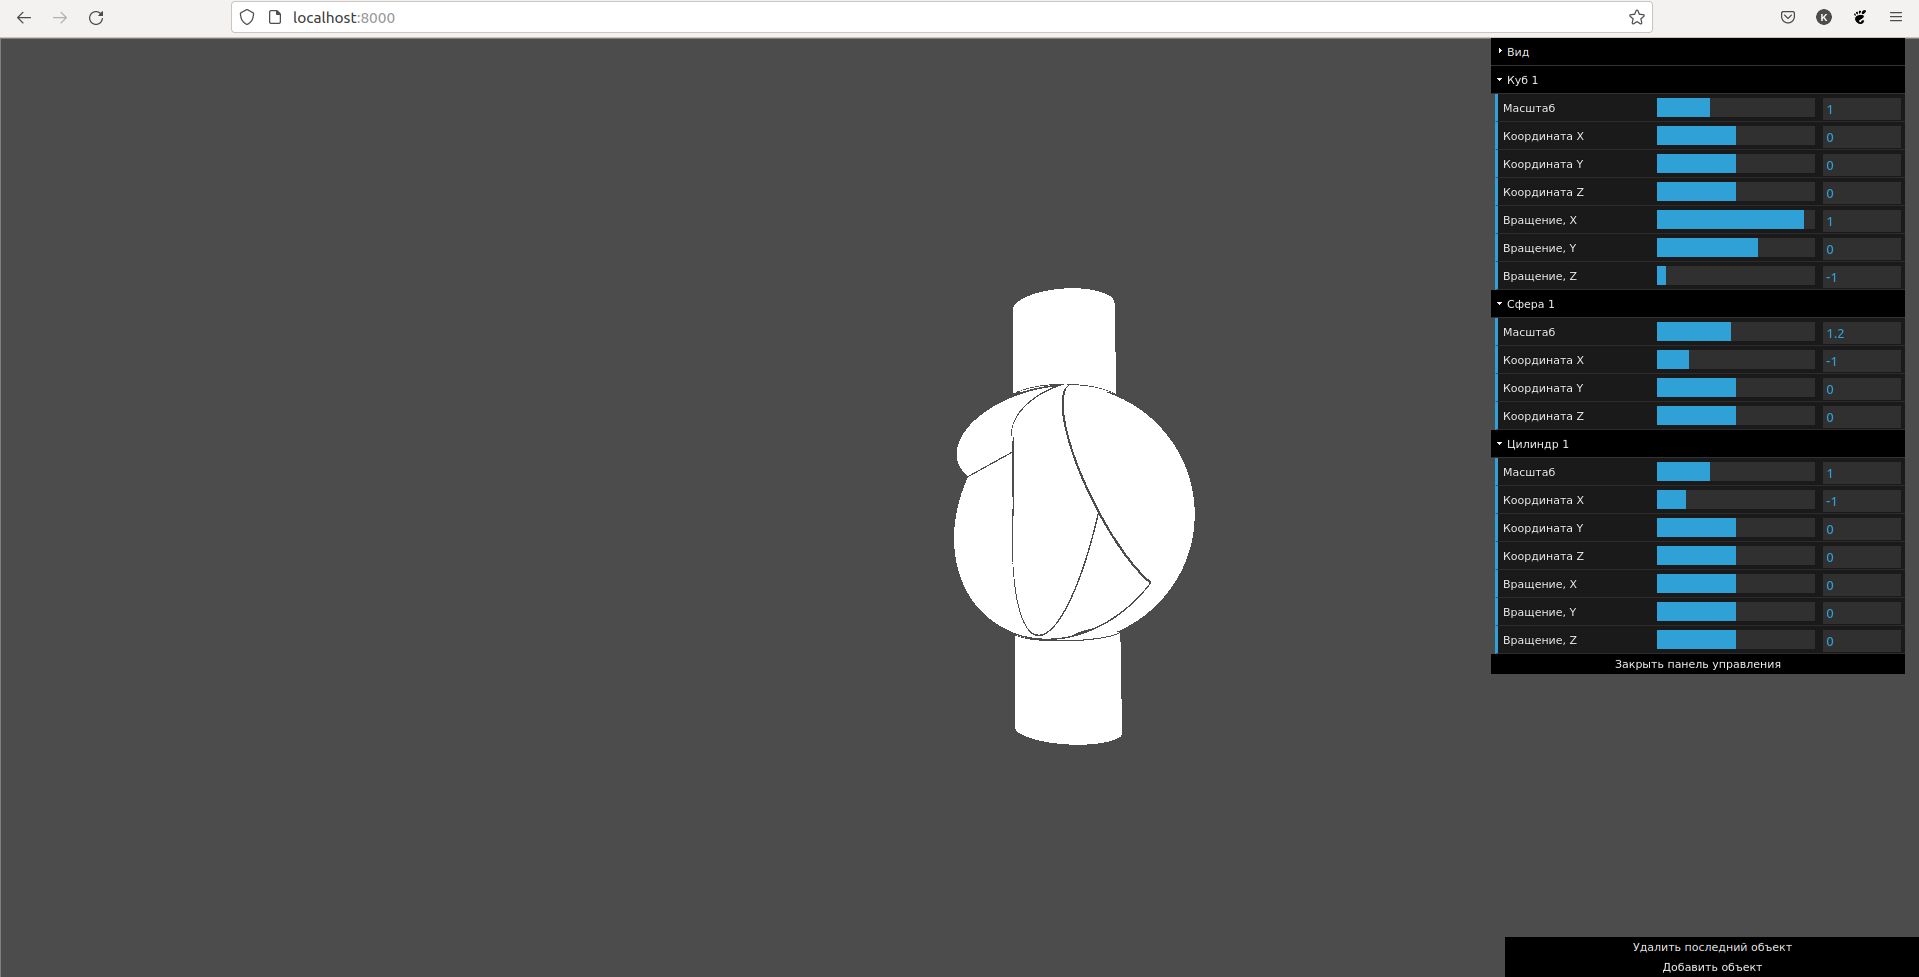
\includegraphics[width=150mm]{img/example-app.png}
	\caption{Демонстрация  работы  программы  (композиция  моделей 
		куба, сферы и цилиндра).}
	\label{fig:example}
\end{figure}


\subsection*{Вывод}
В данном разделе были рассмотрены средства реализации ПО, приведены 
листинги исходного кода программы, разработанной на основе 
алгоритмов,  выбранных  в  аналитическом  разделе  и  изложенных  в 
конструкторском разделе.

\pagebreak